\documentclass[a4paper, fontsize=14pt]{article}
\usepackage{scrextend}
\usepackage{indentfirst, fancyhdr, amsfonts, mathtools, amssymb}
\usepackage{titlesec} %работа с рубрикацией
\usepackage{tocloft} %настройки оглавления
\usepackage[T2A]{fontenc}
\usepackage[utf8x]{inputenc}
\usepackage[russian]{babel}
\usepackage{hyperref} %кликабельное оглавление
\usepackage[left=3.7cm,right=2cm,top=2cm,bottom=2cm]{geometry}
\usepackage{tempora} %настраиваем шрифт типа TNR                                   
\usepackage{newtxmath} %делаем шрифт формул похожим на TNR
\usepackage{caption}
\usepackage{pdfpages}
\usepackage{listings}
\lstset{
  columns=fullflexible,
  breaklines=true,
}
\linespread{1}
\setcounter{page}{4} %в зависимости от того, какой по счёту страницей должно быть оглавление!

%НАСТРОЙКИ ОГЛАВЛЕНИЯ
\renewcommand{\cftsecaftersnum}{.} %точки после номеров разделов и подразделов в оглавлении
\renewcommand{\cftsubsecaftersnum}{.}
\renewcommand{\cftsecfont}{\normalfont} %разделы в оглавлении пишутся обычным (не жирным) шрифтом
\renewcommand{\cftsecpagefont}{\normalfont} %соответствующие им страницы тоже
\renewcommand{\cftsecleader}{\cftdotfill{\cftdotsep}} %расставляем точки между названиями разделов и их страницами
\addto\captionsrussian{\renewcommand\contentsname{СОДЕРЖАНИЕ}} %хотим, чтобы слово "Содержание" писалось капсом
\renewcommand{\cfttoctitlefont}{\hfil\bfseries} %слово СОДЕРЖАНИЕ по центру жирным
\renewcommand{\cftaftertoctitle}{\hfill}

%НАСТРОЙКИ РУБРИКАЦИИ
\titleformat*{\section}{\center\bf} %названия разделов и подразделов по середине жирным шрифтом
\titleformat*{\subsection}{\center\bf}
\titlelabel{\thetitle.\quad} %название раздела и его номер отделены точкой

%НАСТРОЙКИ БИБЛИОГРАФИИ
\addto\captionsrussian{\renewcommand\refname{СПИСОК ЛИТЕРАТУРЫ}} %хотим, чтобы слова "Список литературы" писались капсом
\makeatletter
\renewcommand{\@biblabel}[1]{#1.} %хотим, чтобы в списке литературы номера источников писались в формате "No. <...>", а не "[No] <...>"
\makeatother

\begin{document}

\includepdf[pages={1}]{src/front_page.pdf}
\textbf{Цель работы:} получить навык приближенного вычисления определенных интегралов.
\subsection*{{Ход работы}}
Во всех задачах требуется вычислить приближенное значение
определенного интеграла
\begin{equation*}
    J[f] = \int_a^b f(x) dx
\end{equation*}
от заданной в индивидуальном задании функции:
\begin{equation}
    \label{eq:individual_func}
    f(x) = \frac{\operatorname{arctg} (x)}{1+x^2}, \quad x \in [0, 2]
\end{equation}
Вычислим точное значение $J[f]$ этого интеграла:
\begin{equation}
    \int_0^2 \frac{\operatorname{arctg} (x)}{1+x^2} dx = \int_0^2 \operatorname{arctg} (x) d(\operatorname{arctg} (x)) = \frac{\operatorname{arctg}^2(2)}{2} \approx 0.612889
\end{equation}
\subsubsection*{Задача №1}
\begin{enumerate}
    \item Написать вычислительную программу на языке программирования C++
    для вычисления интеграла $J[f]$ по квадратурным формулам
    прямоугольников и трапеций на равномерной сетке.
    \item Построить графики зависимости абсолютной погрешности
    $$\Delta = |J - \overline{J}|$$
    вычисления интеграла с использованием обеих формул от количества
    узлов сетки.
    \item Для каждой из квадратурных формул определить минимальное
    количество узлов равномерной сетки, обеспечивающее вычисление
    интеграла с указанной в индивидуальном задании величиной
    абсолютной погрешности $\overline{\Delta}$
\end{enumerate}
\subsubsection*{Решение}
    Формула прямоугольников:
    \begin{equation*}
        J[f] = h \sum_{i=1}^n f\left(\frac{x_{i-1} + x_i}{2}\right)
    \end{equation*}

    Формула трапеций:
    \begin{equation*}
        J[f] = h \frac{f(a) + f(b)}{2} + h \sum_{i=1}^{n-1} f(x_i)
    \end{equation*}
    В ходе лабораторной работы было определено, что минимальным числом узлов равномерной сетки для формул прямоугольника при $\Delta = 0.001$ является $n = 1200$, соответствующая ошибка равна $0.000923261$. 
    Для формул трапеций аналогичные данные составили $n = 900$ и ошибка $0.00098486$.
    Графики ошибок от $n$ приведены на рисунке \ref{fig:rectangle_error} и \ref{fig:trapezoid_error}.
    \begin{center}
        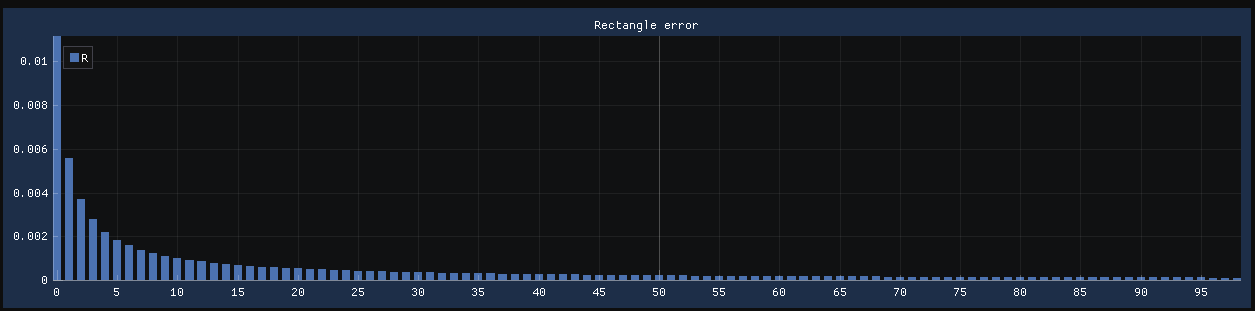
\includegraphics[scale=0.6]{src/rectangle_error.png}
        \captionof{figure}{График ошибки для формулы прямоугольников}
        \label{fig:rectangle_error}
    \end{center}

    \begin{center}
        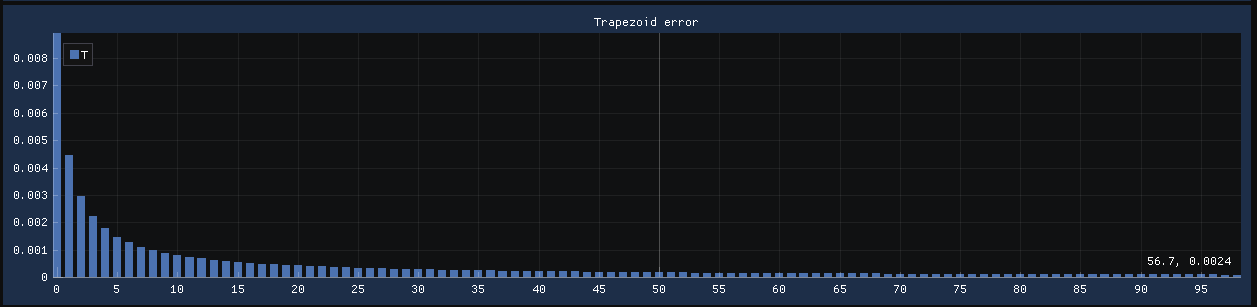
\includegraphics[scale=0.6]{src/trapezoid_error.png}
        \captionof{figure}{График ошибки для формулы трапеций}
        \label{fig:trapezoid_error}
    \end{center}
    \newpage
\subsubsection*{Задача №2}
\begin{enumerate}
    \item Выполнить п. 1)-3) из Задачи 1 для квадратурной формулы Симпсона.
\end{enumerate}
\subsubsection*{Решение}
    Формула Симпсона:
    \begin{equation*}
        J[f] = \frac{h}{3} \left[f(x_0) + 4 \sum_{i=1}^n f(x_{2i-1}) + 2 \sum_{i=1}^{n-1} f(x_{2i}) + f(x_n) \right]
    \end{equation*}
    Для формулы Симпсона были получены результаты: $n = 600$ и ошибка $0.000983762$.
    График ошибки от $n$ приведен на рисунке \ref{fig:simpson_error}.
    \begin{center}
        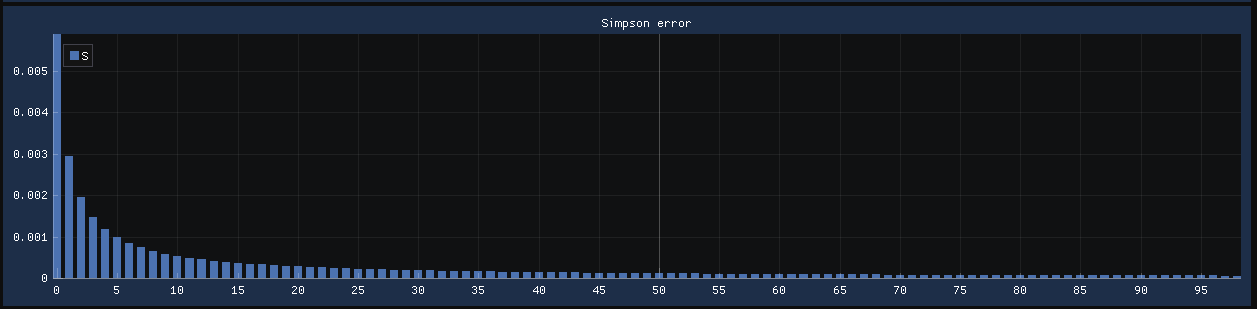
\includegraphics[scale=0.6]{src/simpson_error.png}
        \captionof{figure}{График ошибки для формулы Симпсона}
        \label{fig:simpson_error}
    \end{center}
\subsubsection*{Задача №3}
\begin{enumerate}
    \item С использованием написанной при решении Задачи 1 программы
определить порядок главного члена погрешности квадратуры,
реализовав программно процесс Эйткена.
    \item Зная приближенное значение порядка главного члена погрешности,
    реализовать метод Рунге повышения порядка точности квадратуры.
    Определить порядок точности модифицированного метода.
    \item С использованием правила Ромберга вычислить значение интеграла с
    абсолютной погрешностью $\overline{\Delta} = 10^{-6}$
\end{enumerate}
\subsubsection*{Решение}
Рассмотрим процесс Эйткена, которой на основе повторных просчетов на нескольких сетках дает возможность:
\begin{itemize}
    \item определить фактический порядок точности $q$ квадратурной формулы для заданной подынтегральной функции;
    \item уточнить результат, полученный на исходной сетке.
\end{itemize}

В упрощенном виде процесс Эйткена можно описать следующим образом. 
Выберем три сетки с шагами $h_1 = h, h_2 = h/2, h_3 = h/4$. Вычислим
приближения $I_h$, $I_{h/2}$ и $I_{h/4}$ к интегралу $I$ по выбранной квадратурной
формуле.

Тогда, если учитывать только главный член погрешности, имеем три уравнения для определения $I$, и $q$, где $q$ ~-- фактический, заранее неизвестный порядок точности формулы для данной подынтегральной функции:
\begin{equation*}
    \begin{aligned}
        I &= I_h + O(h^q) \\
        I &= I_{h/2} + \frac{1}{2^q} \alpha h^q \\
        I &= I_{h/4} + \frac{1}{4^q} \alpha h^q
    \end{aligned}
\end{equation*}
в которой значения $I, c, q$ неизвестны. 

Из первого и второго уравнений имеем
\begin{equation*}
    \alpha h^q \left (1 - \frac{1}{2^q}\right) = I_{h/2} - I_h
\end{equation*}

Из второго и третьего уравнений:
\begin{equation*}
    \frac{1}{2^q} \alpha h^q \left (1 - \frac{1}{2^q}\right) =  I_{h/4} - I_{h/2}
\end{equation*}

Из последних двух равенств получаем уравнение для определения $p$:
\begin{equation}
    \label{eq:aitken}
    \begin{aligned}
        2^q = &\frac{I_{h/2} - I_h}{I_{h/4} - I_{h/2}} \\
        q = \operatorname{log_2} &\left( \frac{I_{h/2} - I_h}{I_{h/4} - I_{h/2}} \right)
    \end{aligned}
\end{equation}

Полученную оценку можно использовать для уточнения $I_h$. 

Пусть на $[a, b]$ взята равномерная сетка ${x_i}$ с шагом $h$. Вычислим на
этой сетке приближенное значение $I_h$ интеграла $I$ по какой-либо составной
квадратурной формуле, имеющей алгебраический порядок точности $q = p-1$ (который можно получить из \eqref{eq:aitken}).
Это означает, что имеет место равенство:
\begin{equation}
    \label{eq:runge_1}
    I - I_h = \alpha h^p + O(h^{p+1})
\end{equation}
где в правой части стоит разложение остаточного члена по степеням $h$.

Теперь построим сетку с шагом $h / 2$ и вычислим $I_{h/2}$ по той же самой квадратурной формуле.
Тогда имеем:
\begin{equation*}
    I - I_{h/2} = \overline{\alpha} \left( \frac{h}{2} \right)^p + O\left( \frac{h}{2} \right)^{p+1}
\end{equation*}


Будем считать, что $\alpha \approx \overline{\alpha}$ в силу достаточной малости $h$. Из этих двух равенств ме
можем выразить главный член погрешности $\alpha h^p$ через $I(h)$ и $I_{h/2}$ с точностью $O(h^{p+1})$:
\begin{equation*}
    I_{h/2} - I_h = \alpha h^p - \alpha \frac{h^p}{2^p} + O\left(\left(h^{p+1}\right)\right)
\end{equation*}

Таким образом,
\begin{equation}
    \label{eq:runge_2}
    \alpha h^p = \frac{I_{h/2} - I_h}{1 - 2^{-p}} + O(h^{p+1})
\end{equation}

Подставим теперь \eqref{eq:runge_2} в \eqref{eq:runge_1}. В результате получим новую квадратур-
ную формулу $I_{h,h/2}$ с главным членом погрешности порядка $h_{p+1}$, а не $h_p$,
т.е. вновь полученная формула будет иметь порядок точности на единицу
больше, чем первоначальная формула $I_h$:
\begin{equation*}
        I = I_h + \frac{I_{h/2} - I_h}{1 - 2^{-p}} + \alpha_1 h^{p+1} + O \left(h^{p+2}\right)
\end{equation*}
\begin{equation}
    \label{eq:main_runge}
    I \approx J = I_h + \frac{I_{h/2} - I_h}{1 - 2^{-p}} 
\end{equation}

В ходе лабораторной работы с помощь процесса Эйткена \eqref{eq:aitken} по формуле прямоугольников 
был получен порядок аппроксимации $\overline{p} \approx 1.13$. 
То есть можно принять $p = 1$. Подставим этот результат в формулу \eqref{eq:main_runge}, получим, что ошибка метода составит $3.22\cdot10^{-7}$.

Метод Рунге обобщается на случай произвольного числа сеток, если интегрируемая функция достаточное число раз дифференциуема. Тогда в разложении ТЕйлора можно удерживать большее число членов и подстановка приводит к  представлению остаточного члена в виде ряда:
    \begin{equation*}
        I - I_h = \sum_{m \geq p} \alpha_m h^m 
    \end{equation*}

Пусть расчёт проводится $q$ различных сетках
\begin{equation*}
    I - I_{h/2^j} = \sum_{m = p}^{p + q - 2} \alpha h^m_j + O(h^{p+q-1}) \quad j = 0 \dots q-1
\end{equation*}

Получили СЛАУ относительно $I$ и $\alpha_m$. Отсюда $I$ можно найти по формуле Крамера:
\begin{equation}
    I = \frac{    \det \begin{pmatrix}
        I_{h}&h_1^p&\dots&h_1^{p+q-2} \\
        I_{h/2}&h_2^p&\dots&h_2^{p+q-2} \\
        \dots&\dots&\dots&\dots \\
        I_{h/2^{q-1}}&h_q^p&\dots&h_q^{p+q-2} \\     
    \end{pmatrix}}{    \det \begin{pmatrix}
        1&h_1^p&\dots&h_1^{p+q-2} \\
        1&h_2^p&\dots&h_2^{p+q-2} \\
        \dots  &\dots&\dots&\dots \\
        1&h_q^p&\dots&h_q^{p+q-2} \\
    \end{pmatrix}} + O(h^{p+q-1})
\end{equation}

Эта формула приводит к улучшению точности. Например, при $q = 2$ получаем формулу Ромберга с той же величиной ошибки. 
При $q = 3, \overline{\Delta} =  3.817 \cdot 10^{-11}$, $q=4, \overline{\Delta} = 3.11 \cdot 10^{-14}$.
Однако при больших $q$ ошибка начинает нарастать в виду того,
что при бесконечном уменьшении величины шага, начинает накапливаться машинная погрешность.
\subsubsection*{Задача №4}
\begin{enumerate}
    \item Заменой переменной интегрирования отобразить отрезок
интегрирования $[a,b]$ в $[-1,1]$.
\item Построить квадратурную формулу Гаусса с единичным весом на
системе ортогональных многочленов Лежандра.
\item Выполнить программную реализацию построенной квадратуры на языке программирования С++.
\item С использованием написанной программы построить график
абсолютной погрешности приближенного вычисления интеграла от
числа узлов сетки и определить минимальное количество узлов сетки,
обеспечивающее вычисление интеграла с указанной в индивидуальном
задании величиной абсолютной погрешности $\overline{\Delta}$
\end{enumerate}
\subsubsection*{Решение}
    При заданном числе $N+1$ узлов необходимо построить квадратурную формулу, точную для многчленов наиболее высокой степени.
    
    Построим формулы Гаусса для стандатного отрезка $[-1, 1]$:
    \begin{equation}
        \label{eq:gauss_t}
        \int_{-1}^1 f(t) \approx \sum_{i = 0}^N a_i f(t_i)
    \end{equation}

    Затем с помощью замены переменной $x = \frac{a+b}{2} + \frac{b - a}{2} t$ осуществим переход 
    к формуле интегрирования на произвольном отрезке:
    \begin{equation}
        \label{eq:gauss_x}
        \int_a^b f(x) dx \approx \frac{b - a}{2} \sum_{i=0}^N a_i f\left( \frac{a+b}{2} + \frac{b - a}{2} t_i\right)
    \end{equation}

    Формула \eqref{eq:gauss_t} верна для многочленов степени $m$ тогда и только тогда, когда она точна для функций $f(t) = 1, t, \dots, t^m$. Это эквивалентно тому, что узлы $t_i$ и веса $a_i$ формулы \eqref{eq:gauss_t}
    удовлетворяют системе нелиненых уравнений:
    \begin{equation}
        \label{eq:gauss_at}
        \sum_{t=0}^n a_i(t)i^k = \int_{-1}^1 t^k dt = \frac{1 - (-1)^{k+1}}{k+1}, \quad k = 0, 1, \dots, m
    \end{equation}

    Решения \eqref{eq:gauss_at} часто приводятся в учебниках в виде табличных значений. По данным из [4] были построены приближения на $[-1, 1]$ при $n = 1 \dots 6$. 
    \begin{equation*}
        \begin{aligned}
            \phi_0 =& 2.0 f(0); \\
            \phi_1 =& f(-0.5773502692) +  f(0.5773502692); \\
            \phi_2 =& 0.5555555556 f(-0.7745966692) +\\
            & + 0.8888888888 f( 0.000000000) \\
                   &+ 0.5555555556  f(0.7745966692) \\
            \phi_3 =& 0.3478548451 f(-0.8611363115) + 0.6521451549 f(-0.3399810436) +\\
                   &+ 0.6521451549  f( 0.3399810436) + 0.3478548451  f(0.8611363115)\\
            \phi_4 =& 0.2369268851 f(-0.9061798459) + 0.4786286705 f(-0.5384693101)+ \\
                   &+ 0.5688888888  f( 0.0) + 0.4786286705  f( 0.5384693101)+ \\
                   &+0.2369268851  f(0.9061798459)\\
            \phi_5 =& 0.1713244924 f(-0.9324695142)+ 0.3607615730  f(-0.6612093864)+ \\
            & +0.4679139346  f(-0.2386191861)+ 0.4679139346  f( 0.2386191861)+\\
            &+ 0.3607615730 f( 0.6612093864)+ 0.1713244924  f( 0.9324695142);
        \end{aligned}
    \end{equation*}

    $$\int_a^b f(x) dx \approx  \frac{b - a}{2} \phi_i$$

    Величины соответствующих погрешностей приведены ниже:
        \begin{equation*}
            \begin{matrix*}
                n = 1 &\overline{\Delta} = 0.17250902174089910446\\
                n = 2 &\overline{\Delta} = 0.01473235636043002117\\
                n = 3 &\overline{\Delta} = 0.00499995052291601905\\
                n = 4 &\overline{\Delta} = 0.00007070996194813439\\
                n = 5 &\overline{\Delta} = 0.00007998487100668861\\
                n = 6 &\overline{\Delta} = 0.00000610580087145873\\
            \end{matrix*}
        \end{equation*}

    Таким образом, оптимальным является значение $n = 4$. 

    Требуемый график продемонстрирован на рисунке \ref{fig:gauss_data}.
    \begin{center}
        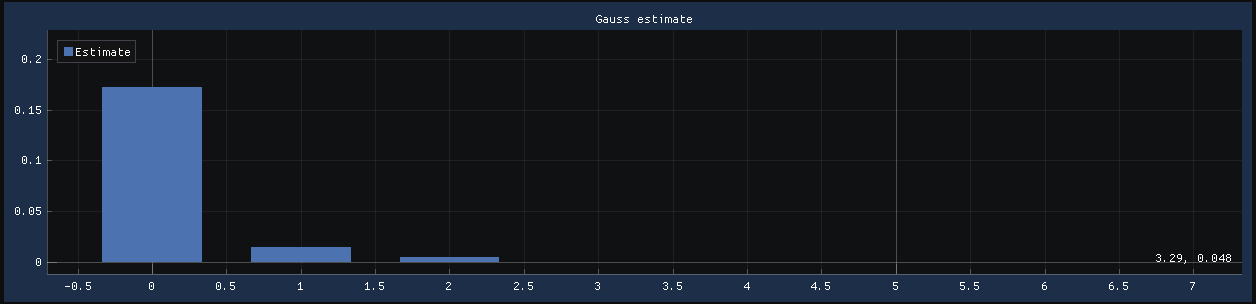
\includegraphics[scale=0.6]{src/gauss.png}
        \captionof{figure}{Зависимость погрешности квадратурной формулы Гаусса от $n$}
        \label{fig:gauss_data}
    \end{center}

\subsubsection*{Задача №5}
\begin{enumerate}
    \item Для заданного интеграла получить приближенное решение задачи об
оптимальном распределении узлов квадратурной формулы трапеций.
    \item Выполнить программную реализацию квадратуры с оптимальным
распределением узлов.
    \item С использованием написанной программы определить минимальное
оптимальное количество узлов сетки, обеспечивающее вычисление
интеграла с указанной в индивидуальном задании величиной
абсолютной погрешности $\overline{\Delta}$.
\end{enumerate}
\subsubsection*{Решение}
    Сетки с равномерными узлами распределения не учитывают особенности подынтегральной функции.
    Попробуем построить адаптивную сетку с заданной точность вычислений $\varepsilon$.
    Пусть $I_0 = 0, x_0 = a, h_1 \leq b - a$, а все значения на $i-1$ шаге уже найдены. Проведем следующий алгоритм: 
\begin{enumerate}
    \item Вычислить \eqref{eq:adapt_trap} \eqref{eq:adapt_control} \eqref{eq:adapt_eps}
    \begin{equation}
        \label{eq:adapt_trap}
        I_{tr, i} = \frac{h_i}{2} ( f(x_{i-1}) + f(x_i) )
    \end{equation}

    \begin{equation}
        \label{eq:adapt_control}
        I_i = \frac{h_i}{4} ( f(x_{i-1}) + 2 f(x_{i-1/2}) + f(x_i)  )
    \end{equation}
    
    \begin{equation}
        \label{eq:adapt_eps}
        \varepsilon_i = \frac{1}{3} (I_i - I_{tr, i})
    \end{equation}
    \item Если $|\varepsilon_i| >  \frac{h_i \varepsilon}{(b - a)}$, то положить $h_i = h_i / 2$ и вернуться к пункту 1.
    \item Если $|\varepsilon_i| \leq \frac{h_i \varepsilon}{(b - a)}$, то вычислить $$x_i = x_{i-1} + h_i$$  $$S_i = S_{i-1} + I_i$$
    \item Если $x_i + h_i > b$, то положить $h_{i+1} = b - x_i$, иначе $h_{i+1} = h_i$. 
    
    На этом $i$-ый шаг завершен.
\end{enumerate}
    В ходе лабораторной работы было получено, что при $n = 30$ получается оптимальное распределение узлов, которое дает погрешность $$ 0.000147 < \varepsilon = 0.001$$
    
    Узлы сетки продемонстрированы на рисунке \ref{fig:adaptive_plot}
   \begin{center}
        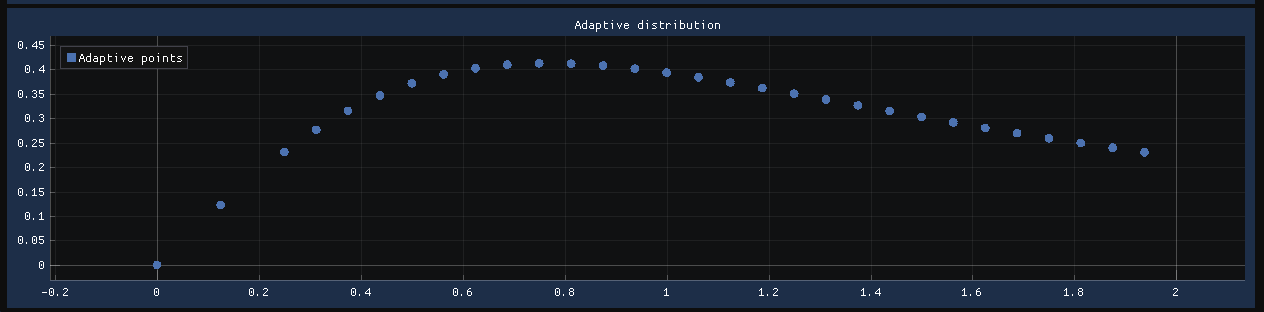
\includegraphics[scale=0.6]{src/adaptive_distribution.png}
        \captionof{figure}{Узлы адаптивной сетки при $n = 30$ функции \eqref{eq:individual_func}}
        \label{fig:adaptive_plot}
    \end{center}
\subsubsection*{Задача №6}
\begin{enumerate}
    \item Написать программу на языке программирования С++ для
приближенного вычисления интеграла методом Монте-Карло.
    \item С использованием написанной программы построить график
    зависимости оценки математического ожидания абсолютной
    погрешности приближенного интегрирования от количества случайных
    точек метода. Размер выборки (количество повторных вычислительных
    экспериментов) для каждого случая принять равным 100.
\end{enumerate}
\subsubsection*{Решение}

Рассмотрим случайную величину $u$, равномерно распределенную на отрезке интегрирования
$[a,b]$ . Тогда $f(u)$ также будет случайной величиной, причем ее математическое ожидание
выражается как 
\begin{equation*}
    M[f(u)] = \int_a^b f(x) \phi(x) dx
\end{equation*}
где $\phi(x)$ плотнотсь распределения случайной величины $u$, равная $\frac{1}{b-1}$ на участке $[a,b]$.
Таким образом, искомый интеграл выражается какой
\begin{equation*}
    \int_a^b f(x) dx = (b - a) M[f(u)]
\end{equation*}
но математическое ожидание величины $f(u)$ можно легко оценить, смоделировав эту
случайную величину и посчитав выборочное среднее.

Итак, бросаем $N$ точек, равномерно распределенных на$[a, b]$, для каждой точки $u_i$ вычисляем
$f(u_i)$. Затем вычисляем выборочное среднее:
\begin{equation*}
    S = \frac{1}{N} \sum_{i=1}^N f(u_i)
\end{equation*}

В итоге получаем оценку интеграла:
\begin{equation*}
    I \approx (b-a) S
\end{equation*}

Трубемый график продемонстрирован на рисунке \ref{fig:montecarlo_plot}.
\begin{center}
    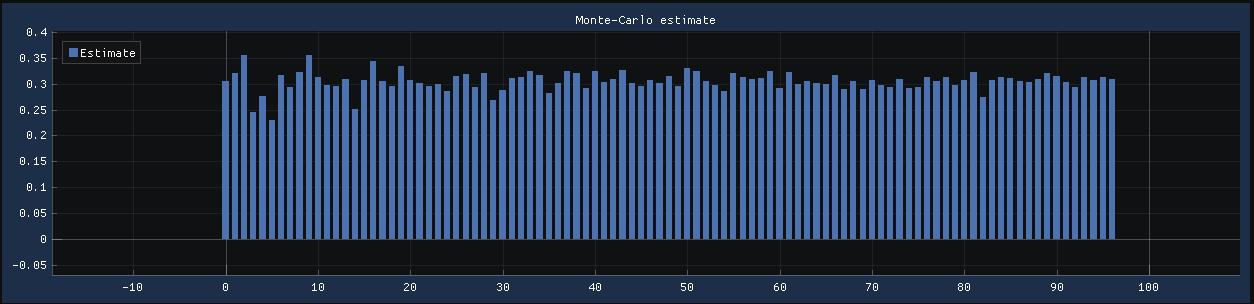
\includegraphics[scale=0.6]{src/monte_carlo_est.png}
    \captionof{figure}{График зависимости оценки математического ожидания абсолютной погрешности приближенного интегрирования от количества случайных точек метода}
    \label{fig:montecarlo_plot}
\end{center}
\newpage
\subsection*{Вывод}
В результате проделанной лабораторной работы был получен навык приближенного вычисления определенных интегралов на языке программирования C++.
\newpage
\subsection*{Список литературы}
\begin{enumerate}
    \item Бахвалов Н.С., Жидков Н.П., Кобельков Г.М. Численные методы: Бином, 2018. – 636 с. 
    \item Калиткин Н.Н. Численные методы, 2-е издание: БХВ-Петербург, 2014. – 592 с.
    \item Самарский А.А., Гулин А. В. Численные методы: Учеб, пособие для вузов, — М.: Наука. Гл. ред. физ-мат. лит., 1989.— 432 с.
    \item А.А. Амосов, Ю.Ф. Дубинский, Н.В. Копчева. Вычислительные методы для инженеров, - М. Высшая школа., 1994.— 273 с.
    \item И. О. Арушанян, Алгоритмы приближенного вычисления интегралов: Учебное пособие, Москва, 2017. - 35 с.
\end{enumerate}
\newpage
\subsection*{Приложение}
Весь код выложен в github-репозитории по ссылке: 

\url{https://github.com/sultanovMF/Numerical-Methods-Lab}

\end{document}


